\section{Turbo Message Passing Framework}
\label{sec:algorithm}

\label{sec:receiver-structure}

Figure~\ref{fig:receiver-structure} shows the factor graph of the posterior in
\eqref{eq:working-posterior}.
Following the turbo message-passing framework in \cite{cai2026}, the receiver
alternates between a linear estimator that exploits the multi-frame
likelihood and a joint denoiser that exploits the channel and activity
priors. The two modules exchange Gaussian extrinsic messages based on
expectation propagation \cite{minka2001}.

\begin{figure}[!t]
\centering
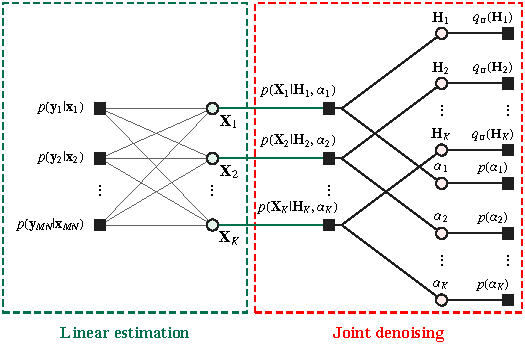
\includegraphics[width=\linewidth]{factor_graph.pdf}
\caption{Factor graph of \eqref{eq:working-posterior} using device blocks
$\mathbf X_k$ as variable nodes. Each likelihood factor depends on the corresponding
column entries from all device blocks. Circles and squares denote
variables and factors. The channel and activity prior branches are
adapted from \cite[Fig.~2]{cai2026}.}
\label{fig:receiver-structure}
\end{figure}

\subsection{Linear Estimation}
\label{sec:linear-estimation}

The linear estimator receives a Gaussian message from joint denoising,
with mean $\mathbf X^{\rm pri}$ and per-column covariance
$\gamma\I_{KN}$, where $\gamma>0$.
Combining this message with the likelihood in \eqref{eq:working-posterior}
gives the posterior mean and covariance
\cite[Sec.~III-A]{cai2026}, \cite[eq.~(15c)]{ma2017}:
\begin{align}
 \mathbf X_{\rm L}
 &=\mathbf X^{\rm pri}
 +\gamma\widehat{\mathbf A}^{\mathsf H}
 (\widehat\sigma^2\I_Q+\gamma\widehat{\mathbf A}\widehat{\mathbf A}^{\mathsf H})^{-1}
 (\mathbf Y-\widehat{\mathbf A}\mathbf X^{\rm pri}),
 \label{eq:linear-mean}\\
 \bm\Sigma_{\rm L}
 &=(\gamma^{-1}\I_{KN}+\widehat\sigma^{-2}\widehat{\mathbf A}^{\mathsf H}\widehat{\mathbf A})^{-1}.
 \label{eq:linear-variance}
\end{align}
The posterior covariance is approximated by
$t_{\rm L}\I_{KN}$, where $t_{\rm L}=\frac{\tr\bm\Sigma_{\rm L}}{KN}$
\cite{ma2015,cai2026}.

The extrinsic message is obtained by dividing this Gaussian approximation
by the incoming message \cite{minka2001}.
Its variance and mean are
\begin{align}
 v_{\rm L}&=(t_{\rm L}^{-1}-\gamma^{-1})^{-1},
 \label{eq:linear-extrinsic}\\
 \mathbf R_{\rm L}&=v_{\rm L}
 \left(\frac{\mathbf X_{\rm L}}{t_{\rm L}}
       -\frac{\mathbf X^{\rm pri}}{\gamma}\right).
 \label{eq:linear-extrinsic-mean}
\end{align}
We partition $\mathbf R_{\rm L}$ by device and pass the resulting matrix blocks
to joint denoising with common variance $v_{\rm L}$.

\subsection{Joint Channel Estimation and Activity Detection}
\label{sec:joint-denoising}

Joint denoising combines the channel estimate under the active hypothesis
with the posterior activity probability to estimate $\mathbf X_k$
\cite[Sec.~III-B]{cai2026}.
For each device, the incoming Gaussian message with mean $\mathbf R_k$
and variance $v$ corresponds to the local observation model
\begin{equation}
 \begin{gathered}
 \mathbf R_k=\alpha_k \mathbf H_k+\mathbf W_k,\\
 \vect(\mathbf W_k)\sim\CN(\mathbf0,v\I_D),
 \end{gathered}
 \label{eq:pseudo-awgn}
\end{equation}
where $\mathbf H_k\sim q_{\rm tr}$ and $D=MN^2$.

\subsubsection{Channel Estimation}
\label{sec:channel-estimation}

Under the active hypothesis $\alpha_k=1$, channel estimation reduces to
denoising the AWGN observation in \eqref{eq:pseudo-awgn}.
The channel prior and Gaussian likelihood determine the conditional mean
and average variance, which we approximate as
\begin{align}
 \mathbf H_k^{\rm post}&\approx
 \E[\mathbf H_k\mid\mathbf R_k,\alpha_k=1],
 \label{eq:conditional-channel-integrals}\\
 t_k&\approx\frac1D\tr\operatorname{Cov}
 (\vect(\mathbf H_k)\mid\mathbf R_k,\alpha_k=1).
 \label{eq:conditional-channel-variance}
\end{align}
Direct evaluation of these moments is difficult because it involves
high-dimensional integrals over $\mathbf H_k$ under the channel prior
$q_{\rm tr}$.

\subsubsection{Activity Detection}
\label{sec:activity-detection}

The inactive and active hypotheses, $\mathbf R_k=\mathbf W_k$ and
$\mathbf R_k=\mathbf H_k+\mathbf W_k$, differ in their observation
distributions. Under the active hypothesis, the likelihood $q_{1,v}$
averages over the unknown channel $\mathbf H$ with prior $q_{\rm tr}$;
under the inactive hypothesis, $q_{0,v}$ is the Gaussian noise density:
\begin{align}
 q_{1,v}(\mathbf R)&=\E[\CN(\vect(\mathbf R);\vect(\mathbf H),v\I_D)],
 \label{eq:query-densities}\\
 q_{0,v}(\mathbf R)&=\CN(\vect(\mathbf R);\mathbf0,v\I_D).
 \label{eq:inactive-density}
\end{align}
With prior activity probability $\rho$, Bayes' rule gives
\begin{equation}
 p^\star(\mathbf R,v)=\frac{\rho q_{1,v}(\mathbf R)}
 {(1-\rho)q_{0,v}(\mathbf R)+\rho q_{1,v}(\mathbf R)}.
 \label{eq:local-activity}
\end{equation}
Computing $q_{1,v}$ requires high-dimensional integration over the unknown
channel, making direct evaluation of this probability difficult.
Let $p_k$ denote the approximation to $p^\star(\mathbf R_k,v)$ used in the joint
estimate below.

\subsubsection{Joint Estimation and Extrinsic Message}
\label{sec:joint-extrinsic}

Combining the activity probability $p_k$ with a Gaussian approximation
to the active-channel posterior, with mean $\mathbf H_k^{\rm post}$
and covariance $t_k\I_D$, gives a Bernoulli--Gaussian approximation
to the posterior of $\mathbf X_k=\alpha_k\mathbf H_k$
\cite[Secs.~III-C--III-D]{liu2018}, \cite[Sec.~III-B]{cai2026}.
Its mean is
\begin{equation}
 \widehat{\mathbf X}_k=p_k\mathbf H_k^{\rm post}.
 \label{eq:mixture}
\end{equation}

Rearranging $\mathbf H_k^{\rm post}$ into
$\mathbf U_k\in\mathbb C^{M\times N^2}$, with one row per antenna,
gives the average posterior covariance across antennas
\begin{equation}
 \mathbf C_{X,k}=p_kt_k\I_M+
 \frac{p_k(1-p_k)}{N^2}\mathbf U_k\mathbf U_k^{\mathsf H}.
 \label{eq:joint-spatial-covariance}
\end{equation}
This covariance accounts for both channel uncertainty under the active
hypothesis and uncertainty in the activity state. Averaging over devices
and antennas gives the posterior variance
\begin{equation}
 \begin{aligned}
 \overline t_X&=\frac{1}{KM}\sum_k\tr\mathbf C_{X,k}\\
 &=\frac1K\sum_k\left[
 p_kt_k+p_k(1-p_k)\frac{\norm{\mathbf H_k^{\rm post}}_F^2}{D}\right].
 \end{aligned}
 \label{eq:joint-average-variance}
\end{equation}

The joint estimate is represented by a Gaussian approximation with mean
$\widehat{\mathbf X}_k$ and common variance $\overline t_X$.
As in \eqref{eq:linear-extrinsic}--\eqref{eq:linear-extrinsic-mean},
division by the incoming Gaussian message gives the extrinsic variance
and mean, with $b=\overline t_X/v$:
\begin{align}
 \gamma_{\rm out}&=\frac{vb}{1-b},
 \label{eq:nonlinear-extrinsic}\\
 \mathbf X_{k,\rm out}&=\frac{\widehat{\mathbf X}_k-b\mathbf R_k}{1-b}.
 \label{eq:nonlinear-extrinsic-mean}
\end{align}
For $0<b<1$, the extrinsic variance is positive.
The output means form $\mathbf X^{\rm pri}$, and $\gamma_{\rm out}$ is the
input variance of the linear estimator in the next iteration.
Section~\ref{sec:learning} addresses the computation of the conditional
channel moments and activity probability required by these updates.
